% This must be in the first 5 lines to tell arXiv to use pdfLaTeX, which is strongly recommended.
\pdfoutput=1
% In particular, the hyperref package requires pdfLaTeX in order to break URLs across lines.

\documentclass[11pt]{article}

% Change "review" to "final" to generate the final (sometimes called camera-ready) version.
% Change to "preprint" to generate a non-anonymous version with page numbers.
\usepackage{acl}

% Standard package includes
\usepackage{times}
\usepackage{latexsym}

% For proper rendering and hyphenation of words containing Latin characters (including in bib files)
\usepackage[T1]{fontenc}
% For Vietnamese characters
% \usepackage[T5]{fontenc}
% See https://www.latex-project.org/help/documentation/encguide.pdf for other character sets

% This assumes your files are encoded as UTF8
\usepackage[utf8]{inputenc}

% This is not strictly necessary, and may be commented out,
% but it will improve the layout of the manuscript,
% and will typically save some space.
\usepackage{microtype}

% This is also not strictly necessary, and may be commented out.
% However, it will improve the aesthetics of text in
% the typewriter font.
\usepackage{inconsolata}

%Including images in your LaTeX document requires adding
%additional package(s)
\usepackage{graphicx}

% If the title and author information does not fit in the area allocated, uncomment the following
%
%\setlength\titlebox{<dim>}
%
% and set <dim> to something 5cm or larger.

\title{Robotic Instruction for Multiple Agents via Natural Language}

% Author information can be set in various styles:
% For several authors from the same institution:
% \author{Author 1 \and ... \and Author n \\
%         Address line \\ ... \\ Address line}
% if the names do not fit well on one line use
%         Author 1 \\ {\bf Author 2} \\ ... \\ {\bf Author n} \\
% For authors from different institutions:
% \author{Author 1 \\ Address line \\  ... \\ Address line
%         \And  ... \And
%         Author n \\ Address line \\ ... \\ Address line}
% To start a separate ``row'' of authors use \AND, as in
% \author{Author 1 \\ Address line \\  ... \\ Address line
%         \AND
%         Author 2 \\ Address line \\ ... \\ Address line \And
%         Author 3 \\ Address line \\ ... \\ Address line}

\author{Isaac Peterson \\
  \texttt{isaac.peterson@usu.edu} \\\And
  Kaiden McMillen \\
  \texttt{kaiden.mcmillen@usu.edu} \\\And 
  Braxton Geary \\
  \texttt{braxton.geary@usu.edu} 
  }

%\author{
%  \textbf{First Author\textsuperscript{1}},
%  \textbf{Second Author\textsuperscript{1,2}},
%  \textbf{Third T. Author\textsuperscript{1}},
%  \textbf{Fourth Author\textsuperscript{1}},
%\\
%  \textbf{Fifth Author\textsuperscript{1,2}},
%  \textbf{Sixth Author\textsuperscript{1}},
%  \textbf{Seventh Author\textsuperscript{1}},
%  \textbf{Eighth Author \textsuperscript{1,2,3,4}},
%\\
%  \textbf{Ninth Author\textsuperscript{1}},
%  \textbf{Tenth Author\textsuperscript{1}},
%  \textbf{Eleventh E. Author\textsuperscript{1,2,3,4,5}},
%  \textbf{Twelfth Author\textsuperscript{1}},
%\\
%  \textbf{Thirteenth Author\textsuperscript{3}},
%  \textbf{Fourteenth F. Author\textsuperscript{2,4}},
%  \textbf{Fifteenth Author\textsuperscript{1}},
%  \textbf{Sixteenth Author\textsuperscript{1}},
%\\
%  \textbf{Seventeenth S. Author\textsuperscript{4,5}},
%  \textbf{Eighteenth Author\textsuperscript{3,4}},
%  \textbf{Nineteenth N. Author\textsuperscript{2,5}},
%  \textbf{Twentieth Author\textsuperscript{1}}
%\\
%\\
%  \textsuperscript{1}Affiliation 1,
%  \textsuperscript{2}Affiliation 2,
%  \textsuperscript{3}Affiliation 3,
%  \textsuperscript{4}Affiliation 4,
%  \textsuperscript{5}Affiliation 5
%\\
%  \small{
%    \textbf{Correspondence:} \href{mailto:email@domain}{email@domain}
%  }
%}

\begin{document}
\maketitle
\begin{abstract}
  In this project, we explore the application of reinforcement learning (RL) to train agents capable of navigating a 2D grid environment and identifying geometric shapes with distinct colors. The agent recieves instruction via natural langauge and then the agents move one space at a time across the grid, using RL techniques to learn an optimal policy for efficiently locating and identifying shapes such as green triangles and red squares. We define the task as a partially observable Markov decision process (POMDP), where the agent's observations are limited to the grid space it occupies. Our approach involves implementing Reinforcement Learning to teach the agents to maximize reward by minimizing the time and steps required to find and correctly identify a shape. The results demonstrate how reinforcement learning can be applied to shape recognition and navigation tasks, with potential applications in robotics, search-and-rescue missions, and autonomous systems. We hope to explore the challenges that come from the multi-agent natural language task completion problema and present viable solutions.

\end{abstract}

\section{Introduction}
As technologies continue to advance, the integration of robots into every day life is continuing to increase. As humans rely mostly on speech for communication and instruction, it is essential that robots are also developed to understand and decipher language, executing commands effectively and efficiently. 

There are a myriad of challenges that one confronts when attempting to solve this problem. First and foremost, establishing an interface between the spoken command and correct execution of that command. To properly execute the spoken command, the agent needs to have an accurate understanding of its environment, which in the real world can become extremely complex, and the connection between the environment and the spoken language. Initial attempts were made by utilizing more logic based methods to help the robot understand the task that needs to be solved \cite{Liu2016}. To mitigate the challenges that come with real world interpretation, many researchers defaulted to simulations to instruct agents in a more structured world \cite{Wang2024}.

Video games form a natural challenge for agents, with clear tasks to complete in a very structured world. \cite{Chaplot2017} used the environment in the video game DOOM\texttrademark ~ to train their agent to follow natural language instructions, with other researchers using similiary techniques in Minecraft\texttrademark ~ \cite{Tessler2020}, and even developing their own virtual environments for natural language task completion \cite{Anderson2017} \cite{Wang2024}. 

Our goal is to use the simplified environment in Minigrid \cite{MinigridMiniworld23} to explore the process of natural langauge task completion, with more research on the multi-agent natural language task completion problem. Where instead of instructing a single agent to complete a task, we instruct a fleet of agents and explore the challenges that come with the increased number of agents along solutions to address these challenges. 

\section{Related Work}
\begin{figure*}[!t]
  \centering
  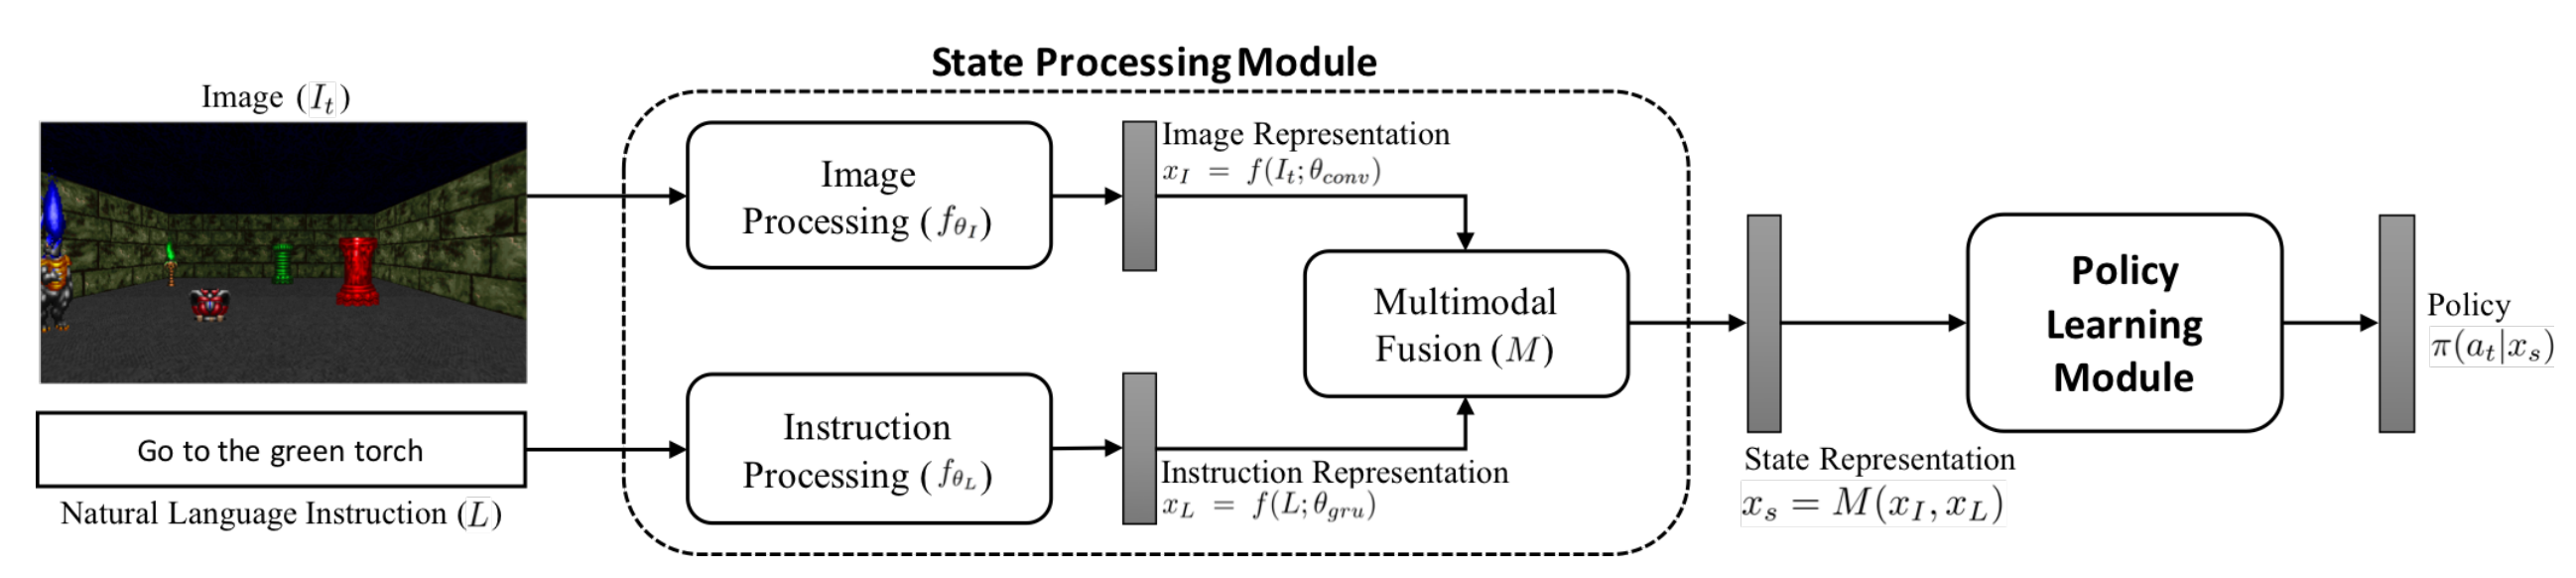
\includegraphics[width=\linewidth]{figs/stateprocessing.png}
  \caption{State processing method as developed by \cite{Chaplot2017}.}
  \label{fig:stateprocess}
\end{figure*}

Most of the work in this project will be based on the work done by \cite{Chaplot2017}. They utilize a combination of large language models and reinforcement learning to help an agent understand specific instructions to navigate in the game environment of doom. Others utilized the world of minecraft to help agents complete tasks, with less of a focus on instruction and more on generalized learning rather than interpreting language \cite{Oh2017}, \cite{Tessler2020}. Combining the implementation of \cite{Chaplot2017} with the Minigrid environment \cite{MinigridMiniworld23}, \cite{chevalier2018babyai} we can further explore the challenging problem of robotic instruction with large language models, with the added challenge of addressing multiple agents.

\section{Methods}

The Minigrid environment is available on a public repository in github which will form the foundation for the environment we will use for the work that we will present in this research. Also foundational to our research is the State Processing Module as shown in Figure~\ref{fig:stateprocess}. Our modified state processing module to use the Minigrid environment and handle multiple agents is shown in Figure~\ref{fig:modeloverview}.



Using notation as described in \cite{Chaplot2017} with slight modification to address our problem, we consider multiple agents interacting with an episodic environment $\Sigma$, at the beginning of each episode, each agent recieves the same natural language instruction $L$, which in our case is a description of the task within the Minigrid environment. At each timestep the agent recieves information about the 8 surrounding blocks around the agent in the environment $E_t$. The episode ends when the agents complete their task or some prefixed maximum time length is met. Let $s_t = (E_t, L)$ represent the state at every timestep, the goal is for the agents to learn the optimal policy $\pi(a_t|s_t)$, which maps the observed states in Minigrid to the optimal next action. 

We will also use the vector representation of the instruction along with a single attention layer to convert the instruction $L$ into a machine interpretable vector $x_L = f_a(L)$. We will use a multi-layer perceptron (MLP) to interpret the grid environment, where $e$ is a vector of length 8 x $n$ representing the 8 blocks surrounding the agent, and $n$ being equal to the number of agents, and the result after being passed through the MLP is $x_E = f_{mlp}(e)$. We concatenate these two vectors together to get our output vector $X = [x_L||x_E]$ which we pass onto our reinforcement learning model to update our policy $\pi(a_t|s_t)$.

\section{Expected Experiments}

  
\begin{figure}[!h]
  \centering
  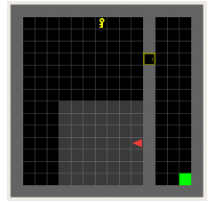
\includegraphics[width=\linewidth]{figs/minigridenv.png}
  \caption{Example of a minigrid level.}
  \label{fig:minigrid}
\end{figure}

\begin{figure*}[!t]
  \centering
  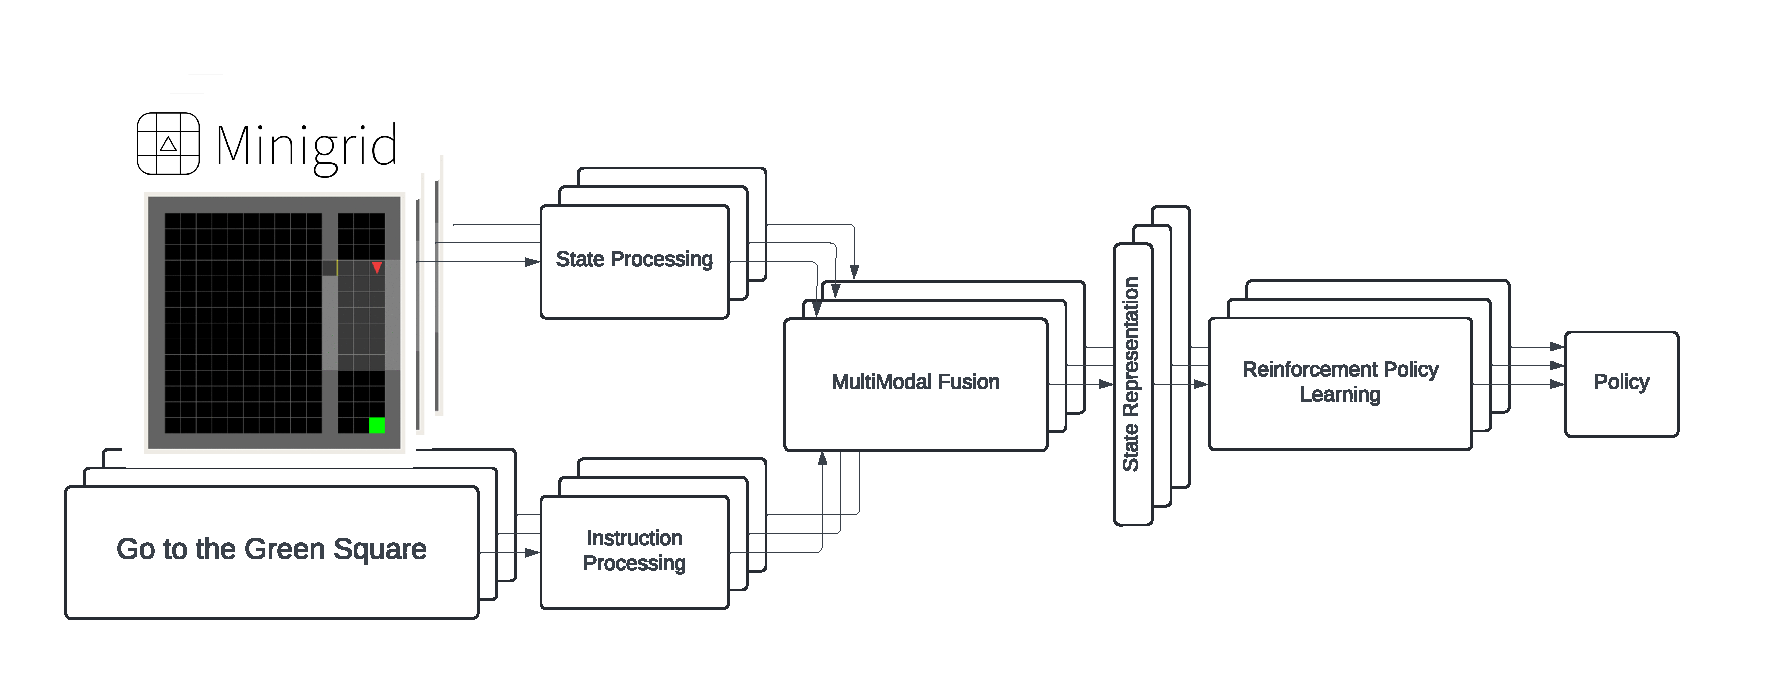
\includegraphics[width=\linewidth]{figs/modeloverviewactual.pdf}
  \caption{Our approach to solving the multi-agent natural language task-solving problem, showing layers for each agent.}
  \label{fig:modeloverview}
\end{figure*}

Since reinforcement learning is an online learning model, we only require the environment as the data to be explored and used to train our model. As mentioned previously we will be using the Minigrid environment to accomplish this task. However, we will have to handcraft some scenarios and reward for the multi-agent portion of this research. Typically the minigrid environment was used for a single agent to complete levels by collecting a key and then exiting to the next level via a green square. 


The minigrid environment provides many building blocks for reinforcement learning tasks, such as a reward for each action. We will have to update this reward to handle multiple agents. For example, if we had two agents completing the level in the minimum number of steps, the optimal policy would be for one agent to grab the key, while the other agent waits by the exit until the key is retrieved. We will need to customize the environment in Minigrid so that the agents can learn this type of behavior. In order to establish baselines for our model performance, we will determine the optimal timesteps to complete each task and compare that with the actions taken by the agents. We can even incorporate this into their reward at the end of the epsiode so the agents learn to complete each level in a more optimal manner.



\section{Teamwork}

The design of the framework as shown in Figure~\ref{fig:modeloverview} makes it easy to deligate the tasks into three separate stages for the project. 

\subsection{Environment Setup}

Kaiden McMillen will be in charge of setting up the environment to train the reinforcement learning model. This will include customizing Minigrid a environment as well as the rewards given to be able to handle multiple agents in a single environment. This will insure that the correct state information can be passed to the State Processing module.

\subsection{State Processing Module}
Isaac Peterson will setup the state processing module. This includes handling the state information from the Minigrid environment and the input instruction $L$, passing them through their appropriate models and creating the output vector $X$ to be processed by the reinforcement learning model. 

\subsection{Multi-Agent Reinforcement Learning}

Braxton Geary will develop the Reinforcement Learning (RL) module for our agent using a Deep Q-Network (DQN) integrated with an 
Asynchronous Advantage Actor-Critic (A3C) algorithm \cite{Mnih2016}. The architecture is comprised of an initial fully connected layer, followed by an LSTM layer, 
and a concluding fully connected layer, allowing it to process inputs from the State Processing Module. The module outputs a tuple with a scalar 
critic value and an array of action probabilities. Where the Actor and Critic share the same neural network, the actor's output undergoes a softmax operation 
to yield action probabilities, \( a_t \). Given that the Minigrid environment limits certain actions, we will apply a negative infinity mask to the logits for 
these unavailable actions, ensuring they remain unselected by the agent. To further enhance stability, we will also incorporate a Proximal Policy Optimization (PPO) 
approach, which will strengthen the model's reliability and effectiveness across diverse scenarios.

% \bibliographystyle{plain}

\bibliography{custom}
\end{document}
